\documentclass{article}

\usepackage{graphicx}
\usepackage{hyperref}

\title{Pentest Playground}
\author{Matthew Hall}


\begin{document}

\maketitle

\section{What is Pentest Playground?}

\paragraph{}
Pentest Playground is a collection of virtual machines and virtual networks inside VMware Workstation.
These have been designed to be used by digital security students to learn and practice their skills in penetration testing and performing security audits.

\section{Configuration}

\subsection{Network}

\paragraph{}
The system uses two virtual networks, provided by VMware Workstation.
\texttt{VMnet1} is a host-only network with the address range \texttt{192.168.107.0/24}.
\texttt{VMnet8} is configured by default to use NAT and has the address range \texttt{192.168.58.0/24}.

\begin{figure}[h!]
	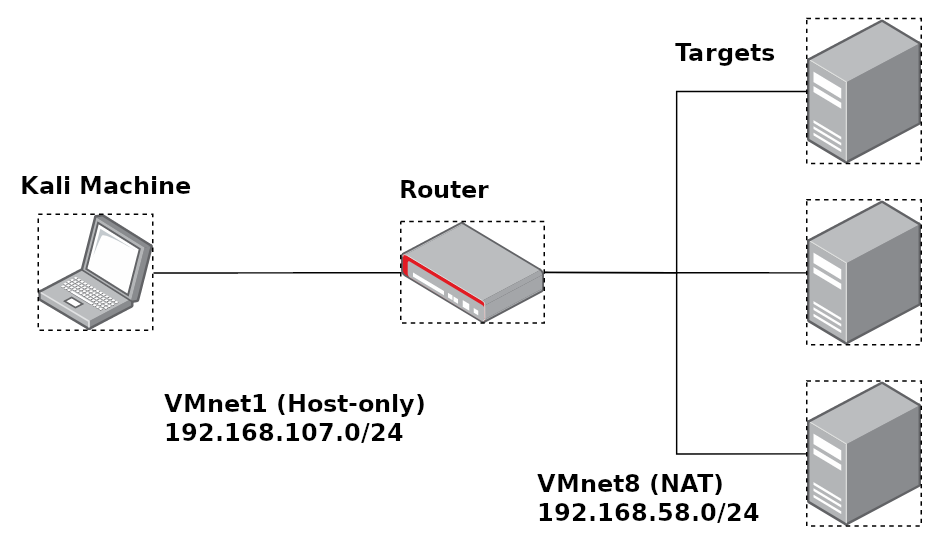
\includegraphics[width=\linewidth]{network.png}
	\caption{Diagram of a possible configuration.}
	\label{fig:network_diagram}
\end{figure}

\paragraph{}
There are two interfaces inside \texttt{VMnet1}.
The first interface belongs to the attacker machine and has a static IP address of \texttt{192.168.107.107}.
The second interface belongs to the router machine and has a static IP address of \texttt{192.168.107.10}.

\paragraph{}
There are an indeterminate amount of interfaces in \texttt{VMnet8}.
One interface belongs to the router machine, with a static IP address of \texttt{192.168.58.10}.
Two other addresses are used by VMware Workstation to allow NAT access to the internet.
The other interfaces on this network will belong to any installed target machines.

\subsection{Machines}

\paragraph{}
The attacker machine is running the LXDE version of Kali Linux\texttrademark \footnote{Kali Linux is a trademark of Offensive Security.} with minimal modification.
The machine has been configured to have a static IP address as described above.
Kali Linux comes with many security related tools, making it ideal for this situation.

\paragraph{}
The router machine in running a minimal installation of Debian GNU/Linux 10 `Buster'.
It has two network interfaces with static IP addresses, as described above.
I has been configured to allow packet forwarding and has routing rules created with \texttt{iptables} to allow the attacker machine to access the the rest of the network.

\paragraph{}
The router machine also has a script that can be run after logging into the router to monitor the traffic of the attacker machine.
The script will launch a container\footnote{\url{https://hub.docker.com/r/hallmatthew314/snort-img}} running Snort, an open-source tool used as a packet-sniffer and IDPS\footnote{Intrusion Detection and Prevention System}.
The specific configuration for Snort will make it monitor the traffic on the router interface on \texttt{VMnet1} where the sender or recipient is the attacker machine.
Whenever it detects a packet, it will display information about the packet to the console.

\section{Intended Use}

\paragraph{}
A user can install target virtual machines into VMware Workstation on the \texttt{VMnet 8} network.
Once a machine is installed and the router and attacker machines are active, the user begin attacking the target machine. If they wish, they can also enable the traffic monitoring to see the packets moving accross the network as they work.

\section{Benefits}

\paragraph{}
While my solution does require the paid version of VMware Workstation for the custom networking, is is not very computationally expensive to run. The total memory requirements for the attacker and router machines is no more than 2 gigbytes, with the only other needed memory being for the target machines.
Additionally, my solution is completely isolated in VMware Workstation, meaning there is a low security risk when using it.

\end{document}
